
\section{Overview of Technology}

In this section an overview of online multiplayer systems is given. For a recent survey of multiplayer online game frameworks we refer the reader to~\cite{Yahyavi:2013:PAM:2522968.2522977}. 

\subsection{Multiplayer Network Design}

To build an online real-time multiplayer game, there are two popular methods.
One, is \ptoP \emph{lockstep}, which is based on the \ptoP architecture.
A diagram of the \ptoP communication structure is shown in Figure~\ref{figure:p2p-vs-ClientServer}(a).
In this approach, all nodes start in the same initial state and each node broadcast every move to the all other nodes.
With nodes communicating directly the \gamestate can not advance until each node's move is received by every other node.
The overall latency of the system is then dependent on the slowest node in the system.
This system is also not tolerant to faulty nodes, as each node will wait and decide themselves if a node has failed.
Since the nodes use broadcasts to communicate, the method generates a significant volume of messages.

To achieve more real-time simulation, systems switched to a \clientServer model (see Figure~\ref{figure:p2p-vs-ClientServer}(b))~\cite{DOOMfaq}. 
With this model the \gamestate is stored on a server and clients send updates to the server.
This model reduces latency, for each client the latency is determined by the connection between that client and the server.
However, this model is still too slow for real-time online multiplayer games, which lead to the introduction of client-side prediction~\cite{bernier2001latency}.
Simply put, client-side prediction allows the client to simulate its own version of the game (sending the results to the server) but the server can still step in and override the client's \gamestate.
This creates complexity in handling server overrides on clients smoothly (not just in code but also in animation and audio).
Another reason for this model to gain traction was the ability to handle malicious clients by validating all actions on the server.


% The \ptoP model does handle fault tolerance more gracefully. Having the single server in the \clientServer model results in little fault tolerance.

	
\begin{figure}[ht]
	\centering
	\begin{tabular}{c c}
		Peer-to-Peer & Client-Server \\
		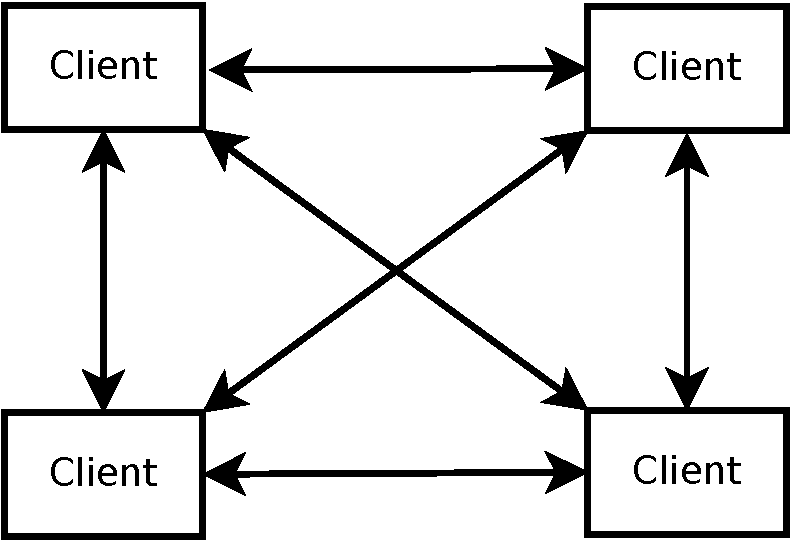
\includegraphics[width=0.48\linewidth]{../images/p2p-model-crop.pdf} &
		%trim=l b r t
		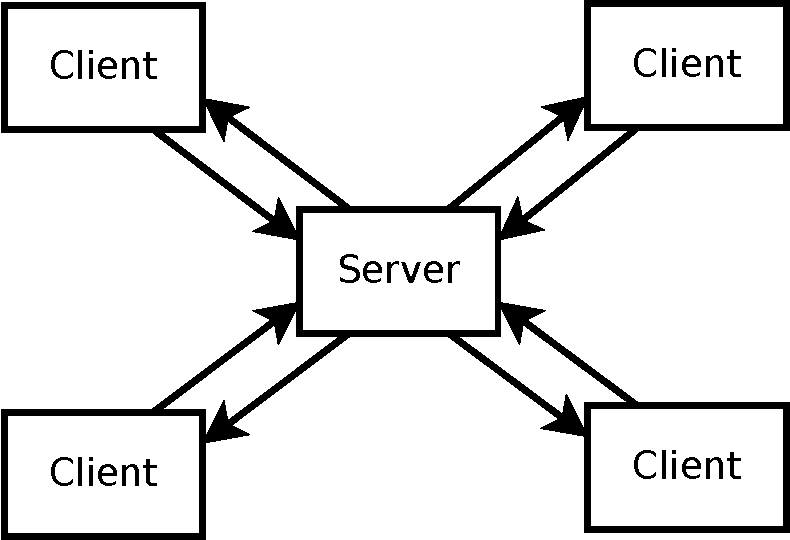
\includegraphics[width=0.48\linewidth]{../images/client-server-model-crop.pdf} \\
		(a) & (b)
	\end{tabular}

	\caption{\label{figure:p2p-vs-ClientServer} Two mutiplayer game networking models. The model on the left (a) is a \ptoP model where every client sends updates directly to ever other client in the game. The second model (b) is a \clientServer model. In this model all of the clients send updates to the server and the server send updates out to the clients.}
	\end{figure}
	
	The system designed in this work uses parts from both the \ptoP model and the \clientServer model. The features of each method that we want to incorporate are:
	\begin{enumerate}
		\item The \clientServer model tends to have less latency
		\item The \clientServer model supports clients joining mid game
		\item The \clientServer model is less susceptible to cheating/malicious clients
		\item The \ptoP model is more fault tolerant
		\item the \ptoP model has distributed state
	\end{enumerate}
	
	As in many multiplayer game networking systems, asynchronous communication is used. This is necessary to preserve the real-time nature of a game. Packet loss is considered not significant as a new packet with more up-to-date information will be sent soon after the lost packet.
	
